%%%%%%%%%%%%%%%%%%
% General config %
%%%%%%%%%%%%%%%%%%

\documentclass{article}
\usepackage[margin=1.2in]{geometry}
\usepackage[english]{babel}

%%%%%%%%%%%%
% Packages %
%%%%%%%%%%%%

% Math packages
\usepackage{amsthm}
\usepackage{amsmath,amssymb}
\usepackage{amsfonts,mathtools}
% \usepackage{thmbox}
\usepackage{bm}
\usepackage{proof-at-the-end}

% graphics packages
\usepackage{pict2e,picture}
\usepackage{graphicx}
\usepackage{tikz}
\usetikzlibrary {positioning,graphs,calc,decorations.pathmorphing,shapes,arrows.meta,arrows,shapes.misc}
\usetikzlibrary{topaths,calc}
\usetikzlibrary{fit}
\usepackage{subcaption}
\usepackage{xcolor}
\usepackage{wrapfig}
\usepackage{float}

% custom environments
\usepackage{comment}
\usepackage{enumitem}
\usepackage{epigraph}
\usepackage{environ}
\usepackage{listings}

% Miscellanious packages
\usepackage{lipsum,mwe,abstract}
\usepackage{multicol}
\usepackage{refcount}
\usepackage{hyperref}
\usepackage{censor}
\usepackage[numbers]{natbib}



%%%%%%%%%%%%%%%%%%%
% Custom Commands %
%%%%%%%%%%%%%%%%%%%

% covering relation
\newcommand{\coveringA}{%
  \mathrel{-\mkern-4mu}<%
}
\newcommand{\coveringB}{\mathrel{\text{$\vcenter{\hbox{\pictcoveringB}}$}}}
\newcommand{\pictcoveringB}{%
  \begin{picture}(1em,.5em)
    \roundcap
    \put(0,.25em){\line(1,0){.6em}}
    \put(.6em,.25em){\line(3,1){.4em}}
    \put(.6em,.25em){\line(3,-1){.4em}}
  \end{picture}%
}

% highlight
\newcommand{\highlight}[1]{%
  \par\noindent
  \colorbox{gray!30}{%
    \parbox{\dimexpr\linewidth-2\fboxsep\relax}{%
      #1
    }%
  }}

% custom theorem environments
\theoremstyle{plain}
\newtheorem{theorem}{Theorem}[section]
\newtheorem{corollary}[theorem]{Corollary}
\newtheorem{lemma}[theorem]{Lemma}
\newtheorem{prop}[theorem]{Proposition}

\theoremstyle{definition}
\newtheorem{definition}[theorem]{Definition}
\newtheorem{example}[theorem]{Example}
\newtheorem{property}[theorem]{Property}
\newtheorem{notation}[theorem]{Notation}
\newtheorem{convention}[theorem]{Convention}
\newtheorem{interpretation}[theorem]{Interpretation}
\newtheorem{remark}[theorem]{Remark}
% \newtheorem{question}[theorem]{Question}
\newtheorem{note}[theorem]{Note}

\newtheorem{question}{Question}
\theoremstyle{plain}
\newtheorem{assertion}{Assertion}[question]

\newenvironment{reponse}{\renewcommand{\proofname}{Réponse}\begin{proof}}{\end{proof}}

% special theorems / definitions / lemmas
\newtheoremstyle{specialthm}% name
{\topsep}%   Space above
{\topsep}%   Space below
{\itshape}%  Body font
{}%          Indent amount
{\bfseries}% Theorem head font
{}%          Punctuation after theorem head -- blank
{0.5em}%     Space after theorem head (0.5em is the default)
{{\thmname{#1}\thmnumber{ #2$^{\bm*}\!$}\thmnote{\ \textmd{(#3)}.}}}

\theoremstyle{specialthm}
\newtheorem{sptheorem}[theorem]{Theorem}
\newtheorem{spcorollary}[theorem]{Corollary}
\newtheorem{splemma}[theorem]{Lemma}
\newtheorem{spprop}[theorem]{Proposition}

% special theorems / definitions / lemmas
\newtheoremstyle{specialdef}% name
{\topsep}%   Space above
{\topsep}%   Space below
{}%  Body font
{}%          Indent amount
{\bfseries}% Theorem head font
{}%          Punctuation after theorem head -- blank
{0.5em}%     Space after theorem head (0.5em is the default)
{{\thmname{#1}\thmnumber{ #2$^{\bm*}\!$}\thmnote{\ \textmd{(#3)}.}}}

\theoremstyle{specialdef}
\newtheorem{spdefinition}[theorem]{Definition}
\newtheorem{spproperty}[theorem]{Property}

% abstract customization
\renewenvironment{abstract}
{\small
  \begin{center}
    \bfseries \abstractname\vspace{-.5em}\vspace{0pt}
  \end{center}
  \list{}{
    \setlength{\leftmargin}{20mm}
    \setlength{\rightmargin}{\leftmargin}
  }
\item\relax}
{\endlist}

% special epigraph/acknowledgements
\newenvironment{dedication}
{\clearpage           % we want a new page
  \vspace*{\stretch{1}}% some space at the top
  \itshape             % the text is in italics
  \raggedleft          % flush to the right margin
  \begin{minipage}{0.6\linewidth}
    \parindent=12pt
  }
  {\end{minipage}
  \par % end the paragraph
  \vspace{\stretch{2}} % space at bottom is three times that at the top
  \raggedleft
  \textit{All Finite Lattices are Algebraic Lattices.}\\
  \textit{-- G. Birkhoff}
  \vspace{\stretch{1}}
  \clearpage           % finish off the page
}

% Size for partition
% \def\Bign#1{\mathclose{\hbox{$\left#1\vbox to11.5\p@{}\right.\n@space$}}\mathopen{}}

% equiv class
\def\equivclass{/}

\title{\Large Lattices} \date{06/16/21}

\begin{document}

\maketitle

% --------------- ABSTRACT
\begin{abstract}

	Definitions, theorems, proofs and examples on lattices: first as ordered sets and then as algebraic structures. Requires knowledge on ordered sets.

\end{abstract}

\docrule

% --------------- MAIN CONTENT

\section{Preliminaries}

\begin{definition}[upper / lower bound] Let $P$ be an ordered set and let $S
\subseteq P$. An element $x \in P$ is an \textbf{upper bound} of $S$ if $s \leq
x$ for all $s \in S$. A \textbf{lower bound} is defined dually. The set of all
upper bounds of $S$ is denoted by $S^{u}$ (read ``S \textbf{upper}'') and the
set of all lower bounds by $S^{l}$ (read ``S \textbf{lower}''). We define them
formally as:
\begin{equation*} S^{u}:=\{x \in P | \forall s \in S, s \leq x\} \text{ and }
S^{l}:= \{x \in P | \forall s \in S, x \leq s\}
\end{equation*}
\end{definition}

\begin{prop} $S^{u}$ is an up-set and $S^{l}$ is a down-set.
\end{prop}

\begin{definition}[least upper / greatest lower bound] If $S^{u}$ has a least
element $x$, then $x$ is called the \textbf{least upper bound}. If $S^{l}$ has a
greatest element $y$, then $y$ is called the \textbf{greatest lower bound}.

The least upper bound of $S$ exists iff:

\begin{quantifiedequation*}{\exists x \in P, \forall y \in P} \forall s \in S, s
\leq y \Leftrightarrow x \leq y
\end{quantifiedequation*}

\begin{remark} For all elements $y \in P$ greater than all elements $s \in S$,
$x$ is the smallest of all the elements $y$.
\end{remark}

Dually, the greatest lower bound of $S$ exists iff:
\begin{quantifiedequation*}{\exists x \in P, \forall y \in P} \forall s \in S, y
\leq s \Leftrightarrow y \leq x
\end{quantifiedequation*}

\begin{remark} For all elements $y \in P$ smaller than all elements $s \in S$,
$x$ is the greatest of all the elements $y$.
\end{remark}

\end{definition}

\begin{remark} The least upper bound of $S$ if also called the
\textbf{suppremum} of $S$, and the greatest lower bound of $S$, the
\textbf{infimum} of $S$. Therefore, the least upper bound will be noted
\textbf{sup} and the greatest lower bound \textbf{inf}.
\end{remark}

\begin{notation} We write $x \lor y$ (read as ``x \textbf{join} y'') in place of
$\sup(\{x,y\})$ when it exists - and $x \land y$ (read as ``x \textbf{meet} y'')
in place of $\inf(\{x,y\})$ when it exists.

Similarly, we write $\bigvee S$ (the ``\textbf{join} of S'') and $\bigwedge S$
(the ``\textbf{meet} of S'') instead of $\sup(S)$ and $\inf(S)$, when these
exist.

If the join or meet is being found in a particular ordered set $P$, in which
case we write $\bigvee_{P}S$ or $\bigwedge_{P}S$.

It is also useful to define a set $S$ according to an indexing set $I$: we have
$S = \{A_i\}_{i \in I}$. In turn, we write the meet for $S$ as $\bigvee_{i \in
I} A_i$ (similarly for join).
\end{notation}

\section{Lattices}

\begin{definition}[lattice / complete lattice] Let $P$ be a non-empty ordered
set.

\begin{enumerate}
\item If $x \land y$ and $x \lor y$ exist for all $x,y \in P$, then $P$ is
called a \textbf{lattice}.
\item If $\bigvee S$ and $\bigwedge S$ exist, for all $S \subseteq P$, then $P$
is called a \textbf{complete lattice}.
\end{enumerate}
\end{definition}

\begin{remark} A more formal (and algebraic) definition of a lattice, which is
build on the propreties of the meet and join operators exists.
\end{remark}

\begin{prop} Let $P$ be any ordered set. If $x,y \in P$ and $x \leq y$, then
$\{x,y\}^u = \uparrow y$ and $\{x,y\}^l = \downarrow x$.
\end{prop}

\begin{proof} To show the two sets are equal, we will show that they are
mutually included in each other.

Let's prove $\{x,y\}^u \subset \uparrow y$.

Let $a \in \{x,y\}^u$. We have $x \leq a$ and $y \leq a$. As such, we have $y
\leq a \implies a \in \uparrow y$.

Let's now prove $\uparrow y \subset \{x,y\}^u$.

Let $a \in \uparrow y$. We have $y \leq a$. Since $x \leq y$ and $y \leq a$, by
transitivity, we have $x \leq a$. So we have $x \leq a$ and $y \leq a$ - which
proves $a \in \{x,y\}^u$.
\end{proof}

\begin{prop} $x \leq y$ if and only if $x \lor y = y$ or $x \land y = x$.
\end{prop}

\begin{proof} Given that $x \leq y$, we know from proposition 5 that $\{x,y\}^u
= \uparrow y$ and $\{x,y\}^l = \downarrow x$. Since the least element of
$\uparrow y$ is $y$ and the greatest element of $\downarrow x$ is $x$, we have
$x \lor y = y$ or $x \land y = x$ whenever $x \leq y$.

Given $x \lor y = y$, we have $\sup(\{x,y\}) = y$ and by definition of $\sup$ we
have $x \leq y$. Same thing for $x \land y$ with the $\inf$.
\end{proof}

\begin{example} Let P be an ordered set.
\begin{center}
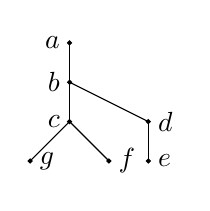
\begin{tikzpicture}[scale=.5] \draw[fill] (0, 3) circle (.05cm) node[left]
{$a$}; \draw[fill] (0, 2) circle (.05cm) node[left] {$b$}; \draw[fill] (0, 1)
circle (.05cm) node[left] {$c$}; \draw[fill] (2, 1) circle (.05cm) node[right]
{$d$}; \draw[fill] (2, 0) circle (.05cm) node[right] {$e$}; \draw[fill] (1, 0)
circle (.05cm) node[right] {$f$}; \draw[fill] (-1,0) circle (.05cm) node[right]
{$g$}; \draw (0,3) -- (0,2); \draw (0,2) -- (0,1); \draw (0,2) -- (2,1); \draw
(2,1) -- (2,0); \draw (0,1) -- (1,0); \draw (0,1) -- (-1,0);
\end{tikzpicture}
\end{center}

We can transform $P$ into a lattice, by ensuring that every pair of elements
have a suppremum and an infimum (since $P$ doesn't have any problems with
non-unique suppremums and infimums). We do this by connecting discrete
``leaves'' into one single element. We will change $a$ into $\top$ (we don't
need to add a new $\top$ element) and add a bottom element $\bot$ which is
covered by $g$, $f$, and $e$.

\begin{center}
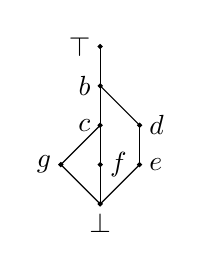
\begin{tikzpicture}[scale=.5] \draw[fill] (0, 3) circle (.05cm) node[left]
{$\top$}; \draw[fill] (0, 2) circle (.05cm) node[left] {$b$}; \draw[fill] (0, 1)
circle (.05cm) node[left] {$c$}; \draw[fill] (1, 1) circle (.05cm) node[right]
{$d$}; \draw[fill] (1, 0) circle (.05cm) node[right] {$e$}; \draw[fill] (0, 0)
circle (.05cm) node[right] {$f$}; \draw[fill] (-1,0) circle (.05cm) node[left]
{$g$}; \draw[fill] (0,-1) circle (.05cm) node[below] {$\bot$}; \draw (0,3) --
(0,2); \draw (0,2) -- (0,1); \draw (0,2) -- (1,1); \draw (1,1) -- (1,0); \draw
(0,1) -- (0,0); \draw (0,1) -- (-1,0); \draw (-1,0) -- (0,-1); \draw (0,0) --
(0,-1); \draw (1,0) -- (0,-1);
\end{tikzpicture}
\end{center}

\end{example}

\begin{remark} Every lattice must posess a bottom $\bot$ and a top $\top$
element. When considering the entire lattice, we find that its upper bound is
$\top$ ($\bot$ for the lower bound)
\end{remark}

\begin{example} Let's give an example of an ordered set that isn't a
lattice. We'll add a bottom and a top element

\begin{center}
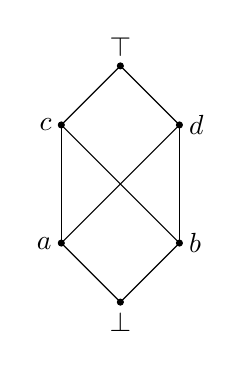
\begin{tikzpicture}[scale=.75] \draw[fill] (0, 3) circle (.05cm) node[above]
{$\top$}; \draw[fill] (-1, 0) circle (.05cm) node[left] {$a$}; \draw[fill] (1,
0) circle (.05cm) node[right] {$b$}; \draw[fill] (-1, 2) circle (.05cm)
node[left] {$c$}; \draw[fill] (1, 2) circle (.05cm) node[right] {$d$};
\draw[fill] (0, -1) circle (.05cm) node[below] {$\bot$}; \draw (-1,0) -- (1,2);
\draw (-1,0) -- (-1,2); \draw (1,0) -- (-1,2); \draw (1,0) -- (1,2); \draw
(-1,2) -- (0,3); \draw (1,2) -- (0,3); \draw (-1,0) -- (0,-1); \draw (1,0) --
(0,-1);
\end{tikzpicture}
\end{center}

We have $\{a,b\}^u = \{c,d,\top\}$ so $c \leq \top$ and $d \leq \top$ but we
have no order relation between $c$ and $d$. So there is no least upper-bound for
the pair $\{a,b\}$.

Similarly, $\{c,d\}^l$ does not have an unique greatest lower element - so the
greatest lower bound doesn't exist for $\{c,d\}$.
\end{example}

\begin{remark} In an ordered set $P$, the least upper bound $x \lor y$ of
$\{x,y\}$ may fail to exist for two different reasons:
\begin{enumerate}
\item because $x$ and $y$ have no common upper bound. (example 1)
\item because $x$ and $y$ have no least upper bound. (example 2)
\end{enumerate}
\end{remark}

\section{Lattices as algebraic structures}

As said in remark 4.; a more algebraic definition for lattices exists. We will
now define such algebraic structure. The next theorem establishes the
equivalence that exists between our previous definition of a lattice and its
algebraic expression.

\begin{lemma}[The Connecting Lemma] Let $L$ be a lattice and let $a,b \in
L$. The following are equivalent:
	\begin{enumerate}
		\item $a \leq b$
		\item $ a \lor b = b$
		\item $a \land b = a$
	\end{enumerate}
\end{lemma}

\begin{proof} 1. $\Leftrightarrow$ 2. and 1. $\Leftrightarrow$ 3. directly
follows from proposition 3, so we just need to prove 2. $\Leftrightarrow$ 3.

  Let's assume 2. Using 2. $\Leftrightarrow$ 1. we get $a \leq b$, so
$\inf(\{a,b\}) = a$ which gives us $a \land b = a$ by the definition of
$\land$. Dually, we get 1. from 2.
\end{proof}

\begin{theorem} Let $(P;\lor,\land)$ be an algebraic structure composed of a non
empty set $P$, two binary relations (the meet and the join which we will combine
in an $\odot$ notation for simplicity's sake) which satisfy the following
indentities for $x, y, z \in P$:
 	\begin{enumerate}
 		\item $x \odot y = y \odot x$ (Commutative)
 		\item $x \odot (y \odot z) = (x \odot y) \odot z$ (Associative)
 		\item $x \odot x = x$ (Idempotent)
 		\item $x = x \lor (x \land y) = x \land (x \lor y)$ (Absorption)
 	\end{enumerate}

	If $(P;\lor,\land)$ satisfies the previous laws, then $P$ is a lattice.
\end{theorem}

\begin{proof} The commutativty and idempotence laws are directly derived from
the propreties of $\sup$ and $\inf$: $x \lor x = \sup(\{x,x\}) = x$ and $x \lor
y = \sup(\{x,y\}) = \sup(\{y,x\}) = y \lor x$ (dually for $\land$).

	\

	In order to prove the associative law we need to prove that $\sup(\{x,
\sup(\{y,z\})\}) = \sup(\{\sup(\{x,y\}), z\}$. We will prove that for any
$a,b,c$: $\sup(\{a,\sup(\{b,c\})\}) = \sup(\{a,b,c\})$ and use the commutativity
of $\sup$ to conclude.

	\

	By the definition of $\sup$ it is enough to prove that $\{a,
\sup(\{b,c\})\}^u =\{a,b,c\}^u$. We will now write $b \lor c$ instead of
$\sup(\{b,c\})$ for more clarity.

	\

	Let $d \in\{a, b \lor c\}^u$. Then $a \leq d$ and $b \lor c \leq d$. This
last relation also gives us $b \leq d$ and $c \leq d$ by definition of the
$\sup$. Therefore, $d \in\{a,b,c\}^u$. Now let $d \in\{a,b,c\}^u$, we have $a
\leq d$ and $b \leq d$ and $c \leq d$ so $b \lor c\leq d$ and it follows that $d
\in\{a, b \lor c\}$. This proves $\{a,b \lor c\}^u =\{a,b,c\}^u$and therefore
the associative law.

	\

	The absorption law can be derived from the connecting Lemma: $x = x \lor (x
\land y) \Leftrightarrow x \land (x \land y) = x \land y$ (Using
2. $\Leftrightarrow 3.$) which; by the indempotence law and the associative law
we just proved, is equivalent to: $x \land y = x \land y\Leftrightarrow \top$
(always true.) . Dually, we prove $x = x \land (x \lor y)$.
\end{proof}

\begin{notation} When considering a lattice as an ordered set we use $(P;
\leq)$, while if we consider it an algebraic structure we use $(P; \lor, \land)$
\end{notation}

\begin{theorem} Let $(L;\lor,\land)$ be a non-empty set equipped with two binary
operations that satisfy the identities of theorem 3.2.
\begin{enumerate}
\item $\forall a,b \in L$ we have $a \lor b = b$ if and only if $a \land b = a$.
\item if we define $\leq$ on $L$ by $a \leq b$ if and only if $a \lor b = b$,
then $\leq$ is an order relation.
\item With $\leq$ as in 2, $(L;\leq)$ is a lattice in which the original
operations agree with the induced operations, that is $\forall a,b \in L$,
\begin{equation*} a \lor b = \sup(\{a,b\}) \text{ and } a \land b =
\inf(\{a,b\})
\end{equation*}
\end{enumerate}
\end{theorem}

\begin{proof} Let's assume $a \lor b = b$. We have $a = a \land (a \lor b)$ by
absorption, and $a \land (a \lor b) = a \land b$. Now let's assume $a \land b =
a$. We have $b = b \lor (b \land a)$ by absorption, which is equal to $b \lor (a
\land b)$ by commutativity, and $b \lor (a \land b) = b \lor a$.

\

We define $\leq$ in $L$ with the following relationship: $a \leq b \iff a \lor b
= b$. $\leq$ is an order relation if it verifies reflexivity, anti-symmetry and
transitivity. By idempotence, using $\leq$'s definition with $b=a$, we have $a
\lor a = a \iff a \leq a$ - thus we showed reflexivity. By commutativity, we
have $a \lor b = b \lor a$ - since $a \lor b = b$ and $b \lor a = a$ and thus $a
= b$ - which shows anti-symmetry. We have $a \lor c = a \lor (b \lor c)$, and $a
\lor c = (a \lor b) \lor c = b \lor c = c$ by associativity. Thus we have $a
\leq c$ from $a \leq b$ and $b \leq c$, so we have shown transitivity.

\

First let's prove $a \lor b \in \{a,b\}^u$; then we will prove that $a \lor b$
is the smallest element of the up-set. We know that $\{a,b\}^u =\{p \in L | a
\leq p \land b \leq p\}$. In adition, $a \lor a \lor b = a \lor b$ and $ b \lor
a \lor b = a \lor b$ so $a \leq a \lor b$ and $b \leq a \lor b$. This proves
that $a \lor b \in \{a,b\}^u$. Now, let $d \in \{a,b\}^u$. We want to prove that
$a \lor b \leq d$; which is equivalent to $a \lor b \lor d = d$. Given that $d
\in \{a,b\}^u$, $a \lor d = d$ and $b \lor d = d$ the previous equation is
immediatly obtained by commutativity. Thus proving that $a \lor b =
\sup(\{a,b\})$. Dually for $\inf$.

\end{proof}

\section{Sublattices, products and homomorphisms}

\subsection{Sublattices}

\begin{definition}[sublattice] Let $L$ be a lattice and $M \subseteq L$
non-empty. Then $M$ is a \textbf{sublattice} of $L$ if $a,b \in M$ implies $a
\lor b \in M$ and $a \land b \in M$.
\end{definition}

\begin{notation} We denote the collection of all sublattices of $L$ by $SubL$
and let $Sub_0 L = Sub L \cap \emptyset$. Both are ordered by inclusion.
\end{notation}

\begin{interpretation} For a subset of lattice to be a sublattice, we must find
\textbf{in the subset}, for every pair of elements in the subset, the
\textbf{sup and inf} present in the original lattice.
\end{interpretation}

\begin{remark} Every covering relation between two elements present in a subset
of a Lattice entails the existance of a $\sup$ and an $\inf$ for those elements
in the subset. So to check if a subset is a sublattice, we only have to check
the existance of $\sup$ and $\inf$ for non edged elements.
\end{remark}

\begin{example} Let $P$ be the following lattice:
\begin{center}
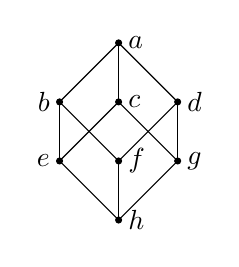
\begin{tikzpicture}[scale=.75] \draw[fill] (0,2) circle (.05cm) node[right]
{$a$}; \draw[fill] (-1,1) circle (.05cm) node[left] {$b$}; \draw[fill] (0,1)
circle (.05cm) node[right] {$c$}; \draw[fill] (1,1) circle (.05cm) node[right]
{$d$}; \draw[fill] (-1,0) circle (.05cm) node[left] {$e$}; \draw[fill] (0,0)
circle (.05cm) node[right] {$f$}; \draw[fill] (1,0) circle (.05cm) node[right]
{$g$}; \draw[fill] (0,-1) circle (.05cm) node[right] {$h$};

\draw (0,2) -- (-1,1); \draw (0,2) -- (1,1); \draw (0,2) -- (0,1); \draw (0,1)
-- (-1,0); \draw (0,1) -- (1,0); \draw (1,0) -- (0,-1); \draw (-1,0) -- (0,-1);
\draw (-1,1) -- (0,0); \draw (1,1) -- (0,0); \draw (0,0) -- (0,-1); \draw (-1,1)
-- (-1,0); \draw (1,1) -- (1,0);
\end{tikzpicture}
\end{center}

We define a subset $P'$ with the following elements: $\{a,b,g,h\}$. This subset
of $P$ is a sublattice since - for any pair of elements in $P'$, $\sup$ and
$\inf$ of any pair of elements is in $P'$. Let's show it in full:
\begin{itemize}
\item For the pairs $\{a,b\}$ and $\{g,h\}$, given one of them covers the other,
it is clear that $\sup$ $\inf$ exist in the subset
\item $\{a,g\}$: $\sup = a$, $\inf = g$
\item $\{a,h\}$: $\sup = a$, $\inf = h$
\item $\{b,g\}$: $\sup = a$, $\inf = h$
\item $\{b,h\}$: $\sup = b$, $\inf = g$
\end{itemize}

Let's now define a subset $P''$ with the following elements: $\{b,e,d,g\}$. This
subset of $P$ isnt a sublattice: for $\{e,g\}$, no $\sup$ or $\inf$ exist in
$P''$ - $\sup(\{e,g\})=c$ and $\inf(\{e,g\})=h$ but $c,h \notin P''$. We could
also show that the suppremum and infimum of $\{b,d\}$ do not exist in $P''$.
\end{example}

\begin{remark} A subset of lattice can be a lattice on its own without being a
sublattice of the original lattice.
\end{remark}

\begin{example} In the lattice $P$ defined in the previous example, if we define
a subset $P'$ with the following elements: $\{a,b,d,e,g,h\}$, we don't obtain a
sublattice: $\sup(\{e,g\}) = c$ and $\inf(\{b,d,\}) = f$ but $c,f \notin P'$.

Nonetheless, if we consider $P'$ by itself, it forms a lattice. (we can find a
$\sup$ and $\inf$ for every pair of elements)
\end{example}


\begin{remark} If two elements $a,b$ such that $a \leq b$ are edged by
transitive closure, it follows that the $\sup(\{a,b\}) = b$ and $\inf(\{a,b\}) =
a$. Otherwise, one has to search for the extremi in the up and down sets
respectively.
\end{remark}

\subsection{Products}

\begin{definition}[products] Let $L$ and $K$ be lattices. Define $\lor$ and
$\land$ coordinate-wise on $L \times K$ as follows:
\begin{align*}
	(l_1, k_1) \lor (l_2,k_2) = (l_1 \lor l_2, k_1 \lor k_2) \\ (l_1,
k_1) \land (l_2,k_2) = (l_1 \land l_2, k_1 \land k_2)
\end{align*}
\end{definition}

\begin{prop} It is customary to check that $L \times K$ verifies the identities
of Theorem 3.2, and is therefore a lattice.

Also,
\begin{align*} (l_1,k_1) \lor (l_2,k_2) = (l_2,k_2) & \iff l_1 \lor l_2 = l_2
\text{ and } k_1 \lor k_2 = k_2 \\ & \iff l_1 \leq l_2 \text{ and } k_1 \leq k_2
\\ & \iff (l_1, k_1) \leq (l_2,k_2)
\end{align*}
\end{prop}

\begin{example}

\end{example}

\begin{remark} Still not sure where it will be useful
\end{remark}

\subsection{Homomorphisms}

\begin{definition}[homomorphism] Let $L$ and $K$ be lattices. A map $f: L
\rightarrow K$ is said to be a \textbf{homomorphism} (or
\textbf{lattice-homomorphism}) if $f$ is \textbf{join-preserving} and
\textbf{meet-preserving}, that is $\forall a,b \in L$:
\begin{equation*} f(a \lor b) = f(a) \lor f(b) \text{ and } f(a \land b) = f(a)
\land f(b)
\end{equation*}

A bijective homomorphism is a (lattice) isomorphism. If $f: L \rightarrow K$ is
a one to one homomorphism (isomorphism), then the sublattice $f(L)$ of $K$ is
isomorphic to $L$ and we refer to $f$ as an \textbf{embedding} (\textbf{of $L$
into $K$})
\end{definition}

\section{Complete lattices, Equivalence Relations, and Algebraic Lattices}

\subsection{Equivalence Relations}

\begin{definition}[equivalence relation] Let $A$ be a set. A binary relation $R$
on $A$ is an \textbf{equivalence relation} on $A$ if, for any $a,b,c \in A$, it
satisfies:
  \begin{enumerate}
  \item $aRa$ (reflexivity)
  \item $aRb$ implies $bRa$ (symmetry)
  \item $aRb$ and $bRc$ imply $aRc$ (transitivity)
  \end{enumerate}

  We denote $Eq(A)$ the set of all equivalence relations on $A$.
\end{definition}

\begin{example} The congruence modulo $n$ defines the following relation: $a =
  kn +b$, for $k \in \mathbb{Z}$. We write $a \equiv b \mod n$.

  We will show that $\equiv$ is reflexive, symmetric and transitive in
  $\mathbb{Z}$

  Let $a,b,c \in \mathbb{Z}$.
  \begin{enumerate}
  \item reflexive ($a \equiv a \mod n$): we have $a = kn + a$ with $k = 0$. As
    such, $a \equiv a \mod n$.
  \item symmetric ($a \equiv b \mod n \implies b \equiv a \mod n$): let's
    suppose $a = kn +b$, then $b = a + (-k)n$. Since $-k \in \mathbb{Z}$,
    we have $b \equiv a \mod n$.
  \item transitive ($a \equiv b \mod n$ and $b \equiv c \mod n$ implies
    $a \equiv c \mod n$): we have $a = kn + b$ and $b = k^{'} n + c$. Therefore,
    $a = kn + (k^{'} n + c) = (k + k^{'})n + c$ and $(k + k^{'}) \in \mathbb{Z}$
    so $a \equiv c \mod n$
  \end{enumerate}
  As such, $\equiv$ is an equivalence relation in $\mathbb{Z}$.
\end{example}

\subsection{Algebraic Lattices}

\begin{definition}[compact element]
	Let $L$ be a lattice. An element $a \in L$ is \textbf{compact} if and only if, for $A \subseteq L$, whenever $\bigvee A$ exists and $a \leq \bigvee A$, then $a \leq \bigvee B$ for some finite $B \subseteq A$.
\end{definition}

\begin{remark}
	Intuitivly, this definition states that whenever $a$ is below the supremum of a set $A$ you can find a finite subset of $A$ that verifies that same property.
\end{remark}

 \begin{remark}
	 All elements of a finite lattice are compact. This is because, for each element $x$ of a finite lattice and for each $A$ such that $x \leq \bigvee A$ (which always exist by the definition of lattice), one can simply chose $B = A$ to prove the existence of a finite subset of $A$ that also satisfies $x \leq \bigvee B$.
 \end{remark}

 \begin{example}
	 If we consider the chain of real numbers. The supremum of the interval $A = ]0,1[$ is 1. However, you cannot find a finite subset $B \subseteq A$ whose supremum is 1: given that $B$ is finite, the supremum of $B$ is $\max B$ which is always lower than 1. If $B$ would have been non-finite it's supremum would indeed be $1$, since it's elements would have been converging towards 1.
\end{example}

 \begin{definition}[compactly generated]
 	A lattice $L$ is \textbf{compactly generated} if and only if every element in $L$ is a sup of compact elements.
 \end{definition}

 \begin{example}
	 The subset $[0,1]$ of a real line is a complete lattice but it nos algebraic, ie. not every element in $[0,1]$ is a sup of compact elements. Indeed, no element of the real chain is compact: consider an element $x \in [0,1]$; then the subset $A = [0,x[$ of $[0,1]$ verifies $x \leq \bigvee A$ as $x = \bigvee A$, but no \textbf{finite subset} B of $A$ exists such that $x \leq \bigvee B$.

     \

     The case $x=1$ is a special case; as $1$ is a sup of all elements of $[0,1]$. But as it was proven that any element in $[0,1[$ is \textbf{not} compact, it is also proven that $[0,1]$ is not compactly generated as $1$ is the sup of entirely non-compact elements (though $1$ is indeed compact in $[0,1]$).

\end{example}

 \begin{remark}
	 All finite lattices are compactly generated. Given that each element of a finite lattice is a sup for other elements (for the bottom case, the sup is the element itself), and that each element of a finite lattice is compact; each element of a finite lattice is a sup of compact elements.
 \end{remark}

\begin{definition}[algebraic lattice]
	A lattice $L$ is \textbf{algebraic} if it is complete and compactly generated.
\end{definition}

\begin{remark}
	All finite lattices are complete.
\end{remark}

\begin{remark}
	\textbf{All finite lattices are algebraic} given remark 5.3 and 5.4
\end{remark}

\section{Closure Operators}

\begin{note}
	test test test
\end{note}






\end{document}
